% Diagram: Encoder-Decoder Architecture
\begin{figure}[htbp]
\centering
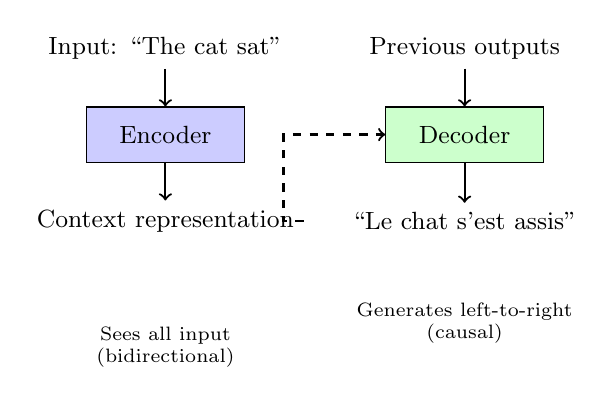
\begin{tikzpicture}[
    node distance=0.8cm,
    block/.style={rectangle, draw, minimum width=2cm, minimum height=0.7cm, font=\small},
    encoder/.style={block, fill=blue!20},
    decoder/.style={block, fill=green!20},
    arrow/.style={->, thick}
]
% Encoder side
\node[encoder] (e1) {Encoder};
\node[above of=e1, yshift=0.3cm] (in) {\small Input: ``The cat sat''};
\node[below of=e1, yshift=-0.3cm] (enc-out) {\small Context representation};

% Decoder side
\node[decoder, right of=e1, xshift=3cm] (d1) {Decoder};
\node[above of=d1, yshift=0.3cm] (prev) {\small Previous outputs};
\node[below of=d1, yshift=-0.3cm] (out) {\small ``Le chat s'est assis''};

% Arrows
\draw[arrow] (in) -- (e1);
\draw[arrow] (e1) -- (enc-out);
\draw[arrow, dashed] (enc-out) -- ++(1.5, 0) |- (d1);
\draw[arrow] (prev) -- (d1);
\draw[arrow] (d1) -- (out);

% Labels
\node[below of=enc-out, yshift=-0.8cm, align=center, font=\scriptsize] {Sees all input\\(bidirectional)};
\node[below of=out, yshift=-0.5cm, align=center, font=\scriptsize] {Generates left-to-right\\(causal)};

\end{tikzpicture}
\caption{Encoder-decoder architecture: encoder summarizes input, decoder generates output.}
\label{fig:encoder-decoder}
\end{figure}
